% !TEX root = /home/eb/.vscode/extensions/qftrules.programme-colle/tmp/Exercice.tex
%%%%%%%%%%%%%%%%%%%%%%%%%%%%%%%%%%%%%%%%%%%%%%%%%%%%%%%%%%%%%%
\begin{exo}[PC][1][devoir]{Éolienne}
%Cet exercice est adapté du sujet d'écrit CCP2 2013, filière PSI.
On assimile une éolienne à ses pales, qui récupèrent une puissance mécanique $\mathcal{P}$ provenant de l'écoulement de l'air avoisinant. On mène l'étude dans le référentiel terrestre supposé galiléen, où les pales sont animées d'un mouvement de rotation uniforme autour de l'axe $(Ox)$ dirigé selon $\vv{e_x}$. Les effets de la pesanteur sont négligés. L'air de masse volumique $\rho$ est assimilé à un gaz parfait et son écoulement autour des pales est supposé stationnaire, parfait, incompressible et à symétrie de révolution autour de l'axe $(Ox)$. On suppose que la vitesse de l'air est uniforme sur une section perpendiculaire au tube de courant passant par les extrémités des pales de l'hélice et représenté ci-dessous. Elle vaut $\vv{V_A}=V_A\,\vv{e_x}$ sur la section $S_A$ située loin en amont des pales et $\vv{V_B}=V_B\,\vv{e_x}$ sur la section $S_B$ située loin en aval des pales. À grande distance des pales, en amont ou en aval, la pression de l'air est uniforme égale à $P_0$. Les sections $\Sigma_1$ et $\Sigma_2$, situées au voisinage immédiat des pales, l'une en amont et l'autre en aval, ont leurs aires quasiment identiques, de sorte qu'on supposera au premier ordre
 $ \Sigma_1 = \Sigma_2 = S $.

La pression du fluide est supposée uniforme sur chacune de ces sections et vaut $P_1$ sur $\Sigma_1$ et $P_2$ sur $\Sigma_2$.
Au voisinage des pales, il y a continuité de la composante normale (selon $\vv{e_x}$) de la vitesse de l'air notée $\vv{V}=V\,\vv{e_x}$. On néglige la dissipation d'énergie par frottement de l'air le long des pales.

%\begin{figure}[h!]
%\centering
\begin{center}

\includegraphics[width=0.47\textwidth]{eolienne.pdf}
\end{center}
%\end{figure}

\begin{quest}
\item Écrire deux relations liant tout ou partie de ces grandeurs: $S_A$, $S_B$, $S$, $V_A$, $V_B$ et $V$. Exprimer ensuite les pressions $P_1$ et $P_2$ en fonction de $P_0$, $\rho$, $V_A$, $V_B$ et $V$. En déduire qu'il existe une discontinuité de la pression au niveau des pales.
\item À partir d'un bilan de quantité de mouvement sur le fluide contenu dans le tube de courant compris entre les sections voisines $\Sigma_1$ et $\Sigma_2$, exprimer la résultante des forces exercée par les pales sur l'air. En déduire l'expression de la puissance $\mathcal{P}$ de la force exercée par l'air sur les pales de l'éolienne en fonction de $\rho$, $S$, $V$, $V_A$ et $V_B$.
\item Retrouver le résultat précédent par un bilan d'énergie cinétique au fluide contenu dans le tube de courant entre les sections $S_A$ et $S_B$.
\item À partir d'un bilan de quantité de mouvement sur le même système qu'à la question 3., établir une deuxième expression de la force exercée par les pales sur l'air. En comparant au résultat précédent, en déduire une relation entre les vitesses $V$, $V_A$ et $V_B$. Exprimer alors la puissance $\mathcal{P}$ en éliminant l'inconnue $V$.
\item Rappeler l'expression du premier principe en terme de puissance pour un système ouvert en régime stationnaire. Justifier le fait que $\Phi_{\rm{th}}=0$ et que $h_{\rm{B}}-h_{\rm{A}}=0$.
\item En posant $x=V_B/V_A$, déterminer la valeur de $x$ pour laquelle $\mathcal{P}$ est maximale. Évaluer la puissance maximale récupérable par une éolienne dont les pales ont un diamètre $D=\SI{60}{m}$ et une vitesse du vent de \SI{40}{km.h^{-1}}. Combien faudrait-il d'éoliennes de ce format, dans les mêmes conditions météorologiques, pour produire la même puissance qu'une tranche de centrale nucléaire de \SI{1,5}{GW} ?
\end{quest}
\end{exo}
%%%%%%%%%%%%%%%%%%%%%%%%%%%%%%%%%%%%%%%%%%%%%%%%%%%%%%%%%%%%%%

%%%%%%%%%%%%%%%%%%%%%%%%%%%%%%%%%%%%%%%%%%%%%%%%%%%%%%%%%%%%%%
\begin{exo}[PC]{Pompe à chaleur}
Une pompe à chaleur permet de maintenir une température constante $T_{\rm{int}}=\SI{20}{\celsius}$ à l'intérieur d'une habitation, la température extérieure étant de $T_{\rm{ext}}=\SI{0}{\celsius}$. Le fluide frigorigène circulant dans la pompe est de l'ammoniac (R717) dont le diagramme entropique est donné ci-dessous. On note $P_{\rm{sat}}(T)$ la pression de vapeur saturante du fluide à la température $T$. On mène toute l'étude en régime permanent. On modélise le cycle thermodynamique du système par l'ensemble de transformations suivantes:
\begin{itemize}
\item[$\bullet$] Entre A et B, le fluide passe dans un échangeur où il est en contact thermique avec l'intérieur de la pièce. Il suit une transformation isobare à la pression de vapeur saturante $P_{\rm{sat}}(T_{\rm{int}})$ au cours de laquelle il ne reçoit pas de travail utile mais échange avec l'intérieur de la pièce un transfert thermique massique $q_{\rm{int}}$. En B le fluide est alors à l'état de liquide saturant à la température $T_{\rm{int}}$.
\item[$\bullet$] Entre B et C, le fluide passe dans un détendeur. Il suit une transformation sans recevoir de travail utile ni transfert thermique. En sortie le fluide est à la pression $P_{\rm{sat}}(T_{\rm{ext}})$.
\item[$\bullet$] Entre C et D, le fluide passe de nouveau dans un échangeur mais cette fois en contact thermique avec l'extérieur. Il suit une transformation isobare à la pression de vapeur saturante $P_{\rm{sat}}(T_{\rm{ext}})$ au cours de laquelle il ne reçoit pas de travail utile mais échange avec l'extérieur un transfert thermique massique $q_{\rm{ext}}$. En D le fluide est alors à l'état de vapeur saturante à la température $T_{\rm{ext}}$.
\item[$\bullet$] Entre D et A, le fluide passe dans un compresseur où il subit une transformation adiabatique réversible au cours de laquelle il reçoit un travail utile massique $w$.
\end{itemize}
%\begin{figure}[h!]
%\centering
\begin{center}

\includegraphics[width=0.9\textwidth]{R717_T_s.jpg}
\end{center}
%\end{figure}
\begin{quest}
\item Par lecture du diagramme entropique, déterminer les valeurs de $P_{\rm{sat}}(T_{\rm{int}})$ et $P_{\rm{sat}}(T_{\rm{ext}})$ puis la valeur de la chaleur latente de vaporisation $\Delta h_{\rm{vap}}$ à $T_{\rm{int}}$ et $T_{\rm{ext}}$.
\item Représenter le cycle ABCD sur le diagramme, et en déduire la valeur de la température en A, notée $T_A$, et celle de la fraction massique de vapeur en C, notée $x_C$.
\item Par lecture graphique, déterminer les valeurs de $w$, $q_{\rm{int}}$ et $q_{\rm{ext}}$. \item Définir et calculer l'efficacité $e$ de la pompe à chaleur, et la comparer à celle de Carnot.
\item Calculer l'entropie massique de fluide créée dans chacun des éléments de la machine et commenter.
\end{quest}
\end{exo}
%%%%%%%%%%%%%%%%%%%%%%%%%%%%%%%%%%%%%%%%%%%%%%%%%%%%%%%%%%%%%%%%%%%%%%%%

%%%%%%%%%%%%%%%%%%%%%%%%%%%%%%%%%%%%%%%%%%%%%%%%%%%%%%%%%%%%%%%%%%%%%
\begin{exo}[PSI][1][devoir]{Force subie par un réservoir}
On considère un réservoir muni d'une vidange.
L'écoulement est homogène, parfait et incompressible. On note $\Vec v_A$ la vitesse (verticale) en entrée et $\Vec v_B$ la vitesse (horiontale) en sortie.


%%% FIGURE : %%%%
%\begin{figure}[h!]
%\centering
\begin{center}

\includegraphics[scale=0.4]{reservoir.png}
\end{center}
%\caption{}
%\label{fig:}
%\end{figure}
%%%%%%%%%%%%%

\begin{quest}

	\item On suppose un régime quasi-stationnaire établi. Montrer
que la vitesse de sortie vaut $v_B = \sqrt{2gh}$ en supposant $v_A \ll v_B$.


	\sol{

Bernouilli avec $p_A=p_B=p_0$ et $v_A \simeq 0$.
  }


	\item Effectuer un bilan de quantité de mouvement sur le volume de fluide contenu dans le réservoir entre deux instants proches $t$ et $t+\d t$. On notera $D_m$ le débit massique de vidange.

	\sol{
	$\d p /\d t = D_m(\Vec v_B-\Vec v_A)$
	}

	\item  On note $\mu$ la masse volumique du fluide. Soit $V$ le volume d'eau contenu dans le récipient et $\Vec F$ la force exercée par l'eau sur le réservoir. Effectuer un bilan des actions extérieures sur ce volume de fluide pour en déduire $\Vec F$.

	\sol{
	$\Vec F = \mu V \Vec g -p_0(S_A\Vec u_z+S_B \Vec u_x)-D_m v_B \Vec u_x$
	}

	\item On s'intéresse maintenant aux actions que subie le réservoir. En définissant une surface fermée fictive, montrer que la résultante des forces de pression de l'air sur le réservoir vaut $\Vec F_p = p_0 S_B \Vec u_x$. Soit $\Vec T$ et $\Vec N$ les réactions respectivement tangentielle et normale du support, et $M$ la masse du récipient. Par un bilan des forces, déterminer $T$ et $N$. Sachant que le réservoir se met à glisser, ce qu'on souhaite éviter, si $T > f N$ avec $f$ le coefficient de frottement, déterminer le débit de vidange maximal.

	\sol{
	$T = D_m v_B$ et $N = mV\mu + M g +p_0 S_A$.
	}

\end{quest}
\end{exo}
%%%%%%%%%%%%%%%%%%%%%%%%%%%%%%%%%%%%%%%%%%%%%%%%%%%%%%%%%%%%%%%%%%%%%%%%%%%%%%%%%


%%%%%%%%%%%%%%%%%%%%%%%%%%%%%%%%%%%%%%%%%%%%%%%%%%%%%%%%%%%%%%%
\begin{exo}[PC]{Charge d'une benne}
Une benne tractée par une force $\vv{F}$ constante possède une masse à vide $m_0$. On néglige tout frottement (ceux de l'air et ceux au niveau du contact avec la route). À l'instant $t=0$, sa vitesse est $v_{\rm{b}}=v_0$ et de plus on verse du sable dans la benne avec un débit massique $D_m$ et avec une vitesse $\vv{v_{\rm{s}}}$ horizontale et constante dans le référentiel lié au sol.
%\begin{figure}[h!]
%\centering
\begin{center}

\includegraphics[width=0.35\textwidth]{camion_sable.pdf}
\end{center}
%\end{figure}
\begin{quest}
\item À l'aide d'un bilan de masse et de quantité de mouvement sur un système que l'on précisera, montrer que la vitesse de la benne évolue selon $v_{\rm{b}}(t)=\frac{m_0v_0+(F+D_m v_{\rm{s}})t}{m_0+D_m t}$.
\item Calculer $\frac{\d E_{\rm{c}}}{\d t}$ avec $E_{\rm{c}}$ l'énergie cinétique de la benne et son contenu, et proposer un bilan de puissance. Commenter.
\end{quest}
\end{exo}

%%%%%%%%%%%%%%%%%%%%%%%%%%%%%%%%%%%%%%%%%%%%%%%%%%%%%%%%%%%%%%%%%%%%%%
\begin{exo}[PC]{Bilan dans un canal}
L'eau d'un canal, de masse volumique $\rho$, s'écoule selon l'axe $(Ox)$. On note $L$ la largeur du canal dans la direction $(Oy)$, et la hauteur d'eau est $h(x,t)$ selon $(Oz)$. On prendra le champ des vitesses de la forme $\vv{v}=v(x,t)\vv{e_x}$.
\begin{quest}
\item Avec la méthode de votre choix, faire un bilan de masse durant $\d t$ sur un système que l'on précisera, et établir l'équation bilan $\frac{\partial h}{\partial t}+\frac{\partial(hv)}{\partial x}=0$.
\item De même, montrer par un bilan de quantité de mouvement que $\frac{\d p_x}{\d t}=\rho L\d x\left(\frac{\partial(hv)}{\partial t}+\frac{\partial(hv^2)}{\partial x}\right)$.
\end{quest}
\end{exo}
%%%%%%%%%%%%%%%%%%%%%%%%%%%%%%%%%%%%%%%%%%%%%%%%%%%%%%%%%%%%%%%%%%%%%%

%%%%%%%%%%%%%%%%%%%%%%%%%%%%%%%%%%%%%%%%%%%%%%%%%%%%%%%%%%%%%%
\begin{exo}[PC]{Le tuyau d'arrosage}
Un tuyau d'arrosage est assimilé à un cylindre rigide de longueur $L$ et de rayon interne $a \ll L$. Une extrémité est fixée en $O$, origine du repère; l'autre est libre et peut pivoter dans le plan $(O,x,y)$. Soit $\theta(t)$ l'angle que fait le tuyau avec l'axe $(Ox)$. De l'eau est injectée dans le tuyau en $O$ et ressort à son autre extrémité; l'écoulement est supposé parfait, incompressible (masse volumique $\rho$) et stationnaire de vitesse $v$ uniforme sur une section du tube. La liaison en $O$ est parfaite et induit sur le tuyau un couple de rappel $\Vec{\Gamma} = - C \theta \Vec{e_z}$ avec $C$ une constante. La pesanteur n'est pas prise en compte dans ce problème. La masse du tuyau est négligée devant la masse de l'eau qu'il contient. L'exercice a pour but de déterminer le mouvement du tuyau, c'est à dire la fonction $\theta(t)$.
%\begin{figure}[h!]
\begin{center}
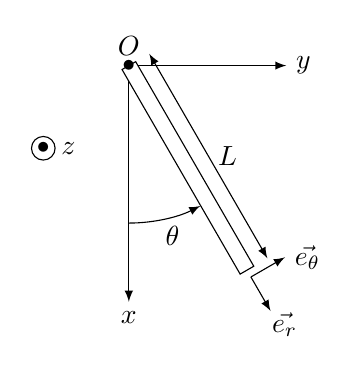
\begin{tikzpicture}

\begin{scope}[rotate=-60]
\coordinate (O) at (0,0.1);
\draw (0,0.1) node[above] {$O$};
\draw[->,>=latex] (3.1,0.1) - ++(0.5,0) node[below right=-3] {$\vec{e_r}$}; 
\draw[->,>=latex] (3.1,0.1) - ++(0,0.5) node[right] {$\vec{e_{\theta}}$}; 
\draw[<->,>=latex] (0,0.4) -- ++(3,0) node[midway, right] {$L$};
\end{scope}

\draw[->,>=latex] (O) -- ++(0,0) --++(2,0) node[right] {$y$};
\draw[->,>=latex] (O) -- ++(0,0) --++(0,-3) node[below] {$x$};

\begin{scope}[rotate=-60]
\fill[white,draw=black] (0,0) rectangle (3,0.2);
\node (O) at (0,0.1) {\small $\bullet$};
\end{scope}

\draw[->,>=latex] (O) ++(0,-2) arc (-90:-63:2) node[below left=4] {$\theta$};

\node (z) at (-1,-1) {\small $\bullet$};
\draw (-1,-1) circle(0.15) node[right=3] {$z$};
\end{tikzpicture}
\end{center}
%\caption{Le tuyau d'arrosage oscille dans le plan $(O,x,y)$. Sa longueur est $L$, son rayon interne $a$ et sa position est repérée par l'angle $\theta(t)$. On introduit la base polaire $(\Vec{e_r}, \Vec{e_{\theta}})$. La liaison en $O$ exerce un couple $\Vec{\Gamma} = - C \theta \Vec{e_z}$.}
%\label{fig:pince}
%\end{figure}


\begin{quest}
\item Montrer que la vitesse $v$ de l'eau dans le référentiel $\mathcal{R}_t$ du tuyau est la même dans toute la longueur du cylindre.
\item Pour déterminer l'équation d'évolution de $\theta(t)$, on se place dans le référentiel terrestre $\mathcal{R}$ supposé galiléen et on effectue un bilan de moment cinétique $\Vec{L_O}$ sur la masse d'eau contenue dans le cylindre. Pour ce faire, il est demandé de définir soigneusement un système fermé à deux instants consécutifs $t$ et $t + \mathrm{d} t$. Celui-ci est constitué d'un volume de contrôle et d'une masse $\mathrm{d}m_1$ entrante à $t$ et $\mathrm{d}m_2=\mathrm{d}m_1=\mathrm{d}m$ sortante à $t + \mathrm{d} t$. Montrer qu'au premier ordre en $\mathrm{d} t$
\begin{equation}
\Vec{L_O}(t+\mathrm{d} t) - \Vec{L_O}(t) = \frac{1}{3}\pi a^2 L^3 \rho \ddot{\theta}(t) \mathrm{d} t \Vec{e_z} + \mathrm{d}m L^2 \dot{\theta}(t) \Vec{e_z}.
\end{equation}
On pourra introduire un point courant du tuyau $M$ de coordonnées polaires $(r,\theta)$ puis intégrer sur toute la longueur du tuyau le moment cinétique élémentaire.
\item En appliquant le théorème du moment cinétique, montrer que $\theta(t)$ satisfait à l'équation
\begin{equation}
\label{eq:theta}
\ddot{\theta} + 2 \lambda \dot{\theta} + \omega_0^2 \theta = 0
\end{equation}
avec $\omega_0 = \sqrt{\frac{3 C}{\pi a^2 L^3 \rho}}$ et $\lambda = \frac{3v}{2L}$. Décrire qualitativement le mouvement du tuyau. Pour quelle valeur $v_c$ de la vitesse $v$ le régime devient-il critique?

\item À partir de l'Éq.~\eqref{eq:theta}, montrer que
\begin{equation}
\label{eq:energ}
\dd{}{t}\left(\frac{1}{2} J \dot{\theta}^2 + \frac{1}{2} C \theta^2 \right) = -m v L \dot{\theta}^2
\end{equation}
où $J=\frac{1}{3}mL^2$ et $m=\pi a^2 L \rho$ est la masse d'eau contenue dans le tuyau à tout instant. Interpréter en terme énergétique. Montrer en particulier que le membre de droite de l'Éq.~\eqref{eq:energ} est le travail effectif de la force de Coriolis $\Vec{F}_{\text{Cor,tuyau}}$ sur le jet d'eau en sortie, ou encore le travail du terme de variation de masse $\dd{m}{t} \Vec{v}$ dans la $2^e$ loi de Newton appliquée au tuyau (système ouvert).

\item On se place dans le référentiel $\mathcal{R}_t$ du tuyau. Effectuer un bilan de quantité de mouvement dans la direction radiale $\Vec{e_r}$ et montrer que pour compenser la force centrifuge, il faut supposer que la pression à l'entrée du tuyau $p_e$ est différente de la pression atmosphérique $p_0$.

\end{quest}
\end{exo}
%%%%%%%%%%%%%%%%%%%%%%%%%%%%%%%%%%%%%%%%%%%%%%%%%%%%%%%%%%%%%%%%%%%%%%%%%%

%%%%%%%%%%%%%%%%%%%%%%%%%%%%%%%%%%%
\begin{exo}[PC][1][TD]{Bilans dans un écoulement stationnaire}
	\Notions{\item Bilan de quantité de mouvement \task Bilan d’énergie}
	On considère l'écoulement stationnaire unidimensionnel d'un fluide dans une conduite à un débit massique $\Dm$. On note $\Vec{v_1}$ et $\Vec{v_2}$ les vitesses en entrée et en sortie de la conduite.
	\begin{quest}
	\item Montrer que la résultante des forces extérieures s'exerçant sur le fluide a pour expression
	% $$
	\begin{equation}
		\Vec{F}_{\rm ext} = \Dm (\Vec{v_2} - \Vec{v_1}).
	\end{equation}
	% $$
	\sol{
		On réalise un bilan de quantité de mouvement sur le système fermé constitué du fluide dans la conduite. On définit $\So$ comme le partie coudée fixe de la canalisation. Le système fermé $\Sf$ mobile, est constitué à l'instant $t$ d'une masse $\d m$ de fluide entrant et de $\So$, et à l'instant $t+\d t$ d'une masse $\d m$ de fluide sortant et de $\So$. La masse $\d m = \Dm \d t$ en entrée et en sortie est la même d'après la stationnarité. Le référentiel $\Rcal$ est celui du laboratoire supposé galiléen.
		On calcule
		\begin{equation*}
		\begin{cases}
		\vv{p}_{\Sf}(t)=\vv{p}_{\So}(t)+\delta\vv{p}_{\rm{e}},\\
		\vv{p}_{\Sf}(t+\d t)=\vv{p}_{\So}(t+\d t)+\delta\vv{p}_{\rm{s}}.
		\end{cases}
		\end{equation*}
		Or  $\delta \Vec{p_{\rm{e}}} = \d m \Vec{v_1} = \Dm \Vec{v_1} \d t$, et de même $\delta\vv{p}_{\rm{s}} = \d m \Vec{v_2} = \Dm \Vec{v_2} \d t$.
		En régime stationnaire, on a $\vv{p}_{\So}(t)=\vv{p}_{\So}(t+\d t)$ et donc
		\begin{equation*}\label{eq:p_stat}
			\vv{p}_{\Sf}(t+\d t) - \vv{p}_{\Sf}(t) = \delta\vv{p}_{\rm{s}} - \delta\vv{p}_{\rm{e}} = \Dm (\Vec{v_2} - \Vec{v_1}) \d t.
		\end{equation*}
		Le PFD appliqué  à $\Sf$ donne ensuite $\vv{p}_{\Sf}(t+\d t) - \vv{p}_{\Sf}(t) = \Vec{F}_{\rm ext} \d t$ et donc
		\eqbox{
			\Vec{F}_{\rm ext} = \Dm (\Vec{v_2} - \Vec{v_1}).
		}
		
	}
	\item Montrer que la puissance totale des forces  s'exerçant sur le fluide a pour expression
	% $$
	\begin{equation}
		\mc{P}_{\rm ext} + \mc{P}_{\rm int} = \frac{1}{2}\Dm (v_2^2 - v_1^2).
	\end{equation}
	% $$
	\sol{
		On réalise un bilan d'énergie mécanique sur le système fermé constitué du fluide dans la conduite. On définit $\So$ comme le partie coudée fixe de la canalisation. Le système fermé $\Sf$ mobile, est constitué à l'instant $t$ d'une masse $\d m$ de fluide entrant et de $\So$, et à l'instant $t+\d t$ d'une masse $\d m$ de fluide sortant et de $\So$. La masse $\d m = \Dm \d t$ en entrée et en sortie est la même d'après la stationnarité. Le référentiel $\Rcal$ est celui du laboratoire supposé galiléen.
		\begin{equation*}
			\begin{cases}
			E_{\rm{c},\Sf}(t)=E_{\rm{c},\So}(t)+\delta E_{\rm{c},\rm{e}},\\
			E_{\rm{c},\Sf}(t+\d t)=E_{\rm{c},\So}(t+\d t)+\delta E_{\rm{c},\rm{s}},
			\end{cases}
			\end{equation*}
			avec $\delta E_{\rm{c},\rm{e}} = \frac{1}{2} \d m v_1^2$ et  $\delta E_{\rm{c},\rm{s}} = \frac{1}{2} \d m v_2^2$.
			Or en régime stationnaire, $E_{\rm{c},\So}(t)=E_{\rm{c},\So}(t+\d t)$ et donc on obtient par différence entre les deux équations $\d E_{\rm{c},\Sf}(t)=\delta E_{\rm{c},\rm{s}}-\delta E_{\rm{c},\rm{e}} = \frac{1}{2} (v_2^2-v_1^2) \Dm \d t$.
			On applique le TEC, ce qui donne
			\begin{equation*}
				\begin{split}
					\frac{\d E_{\rm{c},\Sf}(t)}{\d t}=\mc{P}_{\rm ext} + \mc{P}_{\rm int}
				\end{split}
			\end{equation*}
		et donc
		\eqbox{
			\mc{P}_{\rm ext} + \mc{P}_{\rm int} = \frac{1}{2}\Dm (v_2^2 - v_1^2).
		}
		
	}
\end{quest}
\end{exo}
%%%%%%%%%%%%%%%%%%%%%%%%%%%%%%%%%%%

%%%%%%%%%%%%%%%%%%%%%%%%%%%%%%%%%%%%%%%%%%%%
\begin{exo}[PC][1][TD]{Force exercée par un liquide sur un tuyau coudé}
	\Notions{\item Bilan \task Quantité de mouvement \task Fluide}
On considère un tuyau coudé horizontal de section $S$ constante. L'écoulement de l'eau est homogène, parfait, permanent, incompressible - la masse volumique de l'eau est notée $\mu$. On néglige les variations d'altitude dans le tuyau. On appelle $\Vec{v_1}$ et $\Vec{v_2}$ les vitesses respectivement à l'entrée et à la sortie du tuyau, et $p_1$ et $p_2$ les pressions correspondantes.
\begin{center}

\includegraphics{coude}
\end{center}

\begin{quest}
	\item Justifier que le débit volumique est conservé. Montrer que $v_1=v_2=v$ et $p_1$ = $p_2 = p$.
	\sol{
		Caractérisons tout d'abord les variables de sortie en fonction de celles d'entrée. L'\udl{incompressibilité} de l'écoulement conduit à la conservation du débit volumique, et puisque la section $S=\cte$, on a $v_{\rm{1}}=v_{\rm{2}}=v$. De plus toutes les hypothèses du théorème de \udl{Bernoulli} étant réunies, on peut l'appliquer le long du tube de courant que constitue la canalisation, et il vient alors que 
		\eqbox{
			p_{\rm{1}}=p_{\rm{2}}=p.
		}
	}
	\item On souhaite déterminer la force $\Vec{F}$ exercée sur le tuyau par l'écoulement. Effectuer un bilan de quantité de mouvement entre deux instants $t$ et $t+\d t$ sur une masse donnée d'eau. On définira soigneusement le système fermé étudié.
	\sol{
	On cherche maintenant à évaluer la force exercée par le fluide sur la canalisation. Pour cela, réalisons un bilan de quantité de mouvement dans le référentiel du laboratoire supposé galiléen. Soit $\So$ le système ouvert constitué d'un volume fixe de la conduite qui inclut le coude. On définit le système fermé $\Sf$ par  
	\begin{liste}
		\item $\Sf(t)$ : fluide contenue dans $\So$ + masse $\d m$ entrante entre $t$ et $t+\d t$.
		\item $\Sf(t+\d t)$ : fluide contenue dans $\So$ + masse $\d m$ sortante entre $t$ et $t+\d t$.
	\end{liste}
	Le bilan de quantité de mouvement donne alors
	\begin{equation*}
	\begin{cases}
	\vv{p}_{\Sf}(t)=\vv{p}_{\So}(t)+ \d m\, \Vec{v_1},\\
	\vv{p}_{\Sf}(t+\d t)=\vv{p}_{\So}(t+\d t)+\d m \,\Vec{v_2}.
	\end{cases}
	\end{equation*}
	Or en régime permanent, $\vv{p}_{\So}(t)=\vv{p}_{\So}(t+\d t)$ et donc on obtient par différence entre les deux équations $\d \vv{p}_{\Sf}(t)=\d m (\Vec{v_2}-\Vec{v_1})$, soit d'après le PFD
	% \begin{equation}
		\eqbox{
			\frac{\d \vv{p}_{\Sf}(t)}{\d t} = \mu S v^2\left(\vv{e_y}-\vv{e_x}\right).
			}
	% \end{equation}
	}
	\item En déduire que
	$
	\Vec{F} = S(p+ \mu v^2 )(\Vec{e_y} -\Vec{e_x}).
$
\sol{
On souhaite exprimer une force, on va donc appliquer le PFD au système fermé $\Sf$, soit 
\begin{equation}
\begin{split}
\frac{\d \vv{p}_{\Sf}(t)}{\d t} = \vv{F}_{\rm{can\rightarrow eau}}+
pS(\vv{e_{x}}-\vv{e_{y}})
\end{split}
\end{equation}
On en déduit par action-réaction que 
\eqbox{
\Vec{F} = -\vv{F}_{\rm{can\rightarrow eau}} = S(p+ \mu v^2 )(\Vec{e_y} -\Vec{e_x}).
}
On remarque que cette force est proportionnelle au produit de la surface $S$ par la pression effective $p+\mu v^2$.
}
\end{quest}
\end{exo}
%%%%%%%%%%%%%%%%%%%%%%%%%%%%%%%%%%%%%%%%%%%%

%%%%%%%%%%%%%%%%%%%%%%%%%%%%%%%%%%%
\begin{exo}[PC][2][TD]{Le moulin à eau}
	\Notions{\item Bilan d’énergie \task Bilan de moment cinétique \task Écoulement parfait}
	On étudie le principe d'un moulin à eau. On souhaite déterminer la vitesse de rotation $\omega$ en fonction de la vitesse d'entrée et du couple $\Gamma$ que le fluide exerce sur le moulin. On note $R$ le rayon de la roue du moulin, et $\Dm$ le débit massique du fluide. On suppose que l'eau s'écoule sur une section constante $S$, que l'écoulement est parfait et incompressible, et que la vitesse  du fluide est tangentielle à la roue du moulin.

% \begin{figure}[h!]
\begin{fig}[label]
	\centering
	
\includegraphics[width=0.35\columnwidth]{moulin2.pdf}
	%\capt{}
\end{fig}
	% \centering
	% \caption{Principe du moulin à eau.}
	% \label{fig:bilans_moulin}
% \end{figure}

\begin{quest}
	\item	En appliquant le théorème de l'énergie cinétique (TEC) à un système que l'on précisera, montrer que
	\begin{equation}
	-\Gamma\omega=\frac{1}{2}\Dm\left(v_{\rm{s}}^2-v_{\rm{e}}^2\right),
	\end{equation}
	avec $v_{\rm{e}}$ et $v_{\rm{s}}$ les vitesses d'entrée et de sortie du fluide.
	\item	En appliquant le théorème du moment cinétique (TMC) au même système, montrer que
	\begin{equation}
v_{\rm{s}}=v_{\rm{e}}-\frac{\Gamma}{D_{m}R}.
	\end{equation}
	\item En déduire la caractéristique mécanique $\omega(\Gamma)$ du moulin en fonction de $R$, $S$ et $\Dm$.
\end{quest}

\sol{
\begin{enumerate}
		\item On définit $\So$ comme le partie coudée fixe du jet d'eau. Le système fermé $\Sf$ mobile, est constitué à l'instant $t$ de la partie bleue et de $\So$, et à l'instant $t+\d t$ de la partie rouge et de $\So$. Le référentiel $\Rcal$ est celui du laboratoire supposé galiléen.
		\item On a
		\begin{equation}
		\begin{cases}
		E_{\rm{c},\Sf}(t)=E_{\rm{c},\So}(t)+\delta E_{\rm{c},\rm{e}},\\
		E_{\rm{c},\Sf}(t+\d t)=E_{\rm{c},\So}(t+\d t)+\delta E_{\rm{c},\rm{s}},
		\end{cases}
		\end{equation}
		avec $\delta E_{\rm{c},\rm{e}} = \frac{1}{2} \delta m_{\rm e} v_{\rm e}^2$ et  $\delta E_{\rm{c},\rm{s}} = \frac{1}{2} \delta m_{\rm s} v_{\rm s}^2$.
		\item Or en régime stationnaire, $E_{\rm{c},\So}(t)=E_{\rm{c},\So}(t+\d t)$ et donc on obtient par différence entre les deux équations $\d E_{\rm{c},\Sf}(t)=\delta E_{\rm{c},\rm{s}}-\delta E_{\rm{c},\rm{e}} = \frac{1}{2}\Dm\d t v_{\rm{s}}^2 - \frac{1}{2}\Dm\d t v_{\rm{e}}^2$,
		et donc
		\begin{equation}
		\frac{\d E_{\rm{c},\Sf}(t)}{\d t}=\frac{1}{2}\Dm\left(v_{\rm{s}}^2-v_{\rm{e}}^2\right).
		\end{equation}
		\item On applique le TEC en supposant l'écoulement parfait et incompressible, ce qui donne
		\begin{equation}
			\begin{split}
				\frac{\d E_{\rm{c},\Sf}(t)}{\d t}=\mc{P}_{\rm ext}=-\Gamma\omega.
			\end{split}
		\end{equation}
\end{enumerate}


On admet que l'application du TMC permet de trouver la relation suivante entre les vitesses d'entrée et de sortie,
\begin{equation}
v_{\rm{s}}=v_{\rm{e}}-\frac{\Gamma}{D_{m}R}.
\end{equation}
En combinant les résultats précédents, on en déduit la vitesse angulaire
\begin{equation}
\begin{split}
\omega=\dfrac{v_{\rm{e}}}{R}-\frac{\Gamma}{2R^{2}\Dm}.
\end{split}
\end{equation}
Le moulin tourne d'autant plus vite que la vitesse d'entrée du fluide est élevée, que le rayon de la roue est petit, et que le couple résistant de la roue est faible.
}

\end{exo}
%%%%%%%%%%%%%%%%%%%%%%%%%%%%%%%%%%%


%%%%%%%%%%%%%%%%%%%%%%%%%%%%%%%%%%%%%%%%%%%%
\begin{exo}[PC][3][TD]{Le tourniquet hydraulique}
	\Notions{\item Bilan de quantité de mouvement \task Bilan de moment cinétique \task Écoulement parfait}
On considère un tuyau coudé en angle droit, horizontal, et de section $S$ constante. L'écoulement de l'eau dans ce tuyau est parfait, permanent, incompressible, et la masse volumique de l'eau est notée $\rho$. On appelle $\Vec{v_1}$ et $\Vec{v_2}$ les vitesses respectivement à l'entrée et à la sortie du tuyau, et $p_1$ et $p_2$ les pressions correspondantes.
\begin{center}

\includegraphics{coude}
\end{center}

\begin{quest}
	\item Justifier que le débit volumique est conservé. Montrer que $v_1=v_2=v$ et $p_1$ = $p_2 = p$.
	\sol{
		Caractérisons tout d'abord les variables de sortie en fonction de celles d'entrée. 
		\begin{enumerate}
			\item 
			L'\udl{incompressibilité} de l'écoulement conduit à la conservation du débit volumique $\DV = S v$, et puisque la section $S=\cte$ est constante, on a  
			\eqbox{
				v_{\rm{1}}=v_{\rm{2}}=v.
			}
			
			\item De plus toutes les hypothèses du théorème de \udl{Bernoulli} étant réunies, on peut l'appliquer le long du tube de courant que constitue la canalisation, et il vient alors que 
			\eqbox{
				p_{\rm{1}}=p_{\rm{2}}=p.
				}
			\end{enumerate}
	}
	\item On souhaite déterminer la force $\Vec{F}$ exercée sur le tuyau par l'écoulement de l'eau et l'air environnant. Effectuer un bilan de quantité de mouvement entre deux instants $t$ et $t+\d t$ sur une masse donnée d'eau. On définira soigneusement le système fermé étudié. En déduire que la force recherchée vaut
	 \begin{equation}
		\Vec{F} = \Dm v (\ey - \ex).
	\end{equation}
	\sol{
	On cherche maintenant à évaluer la force exercée par le fluide sur la canalisation. Pour cela, réalisons un bilan de quantité de mouvement dans le référentiel du laboratoire supposé galiléen. Soit $\So$ le système ouvert constitué d'un volume fixe de la conduite qui inclut le coude. On définit le système fermé $\Sf$ par  
	\begin{liste}
		\item $\Sf(t)$ : fluide contenue dans $\So$ + masse $\d m$ entrante entre $t$ et $t+\d t$.
		\item $\Sf(t+\d t)$ : fluide contenue dans $\So$ + masse $\d m$ sortante entre $t$ et $t+\d t$.
	\end{liste}
	Le bilan de quantité de mouvement donne alors
	\begin{equation*}
	\begin{cases}
	\vv{p}_{\Sf}(t)=\vv{p}_{\So}(t)+ \d m\, \Vec{v_1},\\
	\vv{p}_{\Sf}(t+\d t)=\vv{p}_{\So}(t+\d t)+\d m \,\Vec{v_2}.
	\end{cases}
	\end{equation*}
	Or en régime permanent, $\vv{p}_{\So}(t)=\vv{p}_{\So}(t+\d t)$ et donc on obtient par différence entre les deux équations $\d \vv{p}_{\Sf}(t)=\d m (\Vec{v_2}-\Vec{v_1})$, soit 
	% \begin{equation}
		\eqbox{
			\frac{\d \vv{p}_{\Sf}(t)}{\d t} =  \Dm v  (\ex-\ey).
			}
	D'après le PFD, cette grandeur est égale à la résultante des forces extérieures exercées sur le fluide, à savoir la force exercée par le tuyau et celle exercée par l'air ambiant. Or la résultante des forces exercées par l'air sur le fluide et le tuyau est nulle (pression atmosphérique partout). On a donc
	$$
	\frac{\d \vv{p}_{\Sf}(t)}{\d t} = \Vec{F}_{\rm tuyau \rightarrow eau} + \Vec{F}_{\rm air \rightarrow eau} = \Vec{F}_{\rm tuyau \rightarrow eau} - \Vec{F}_{\rm air \rightarrow tuyau} = - \Vec{F}_{\rm eau \rightarrow tuyau} - \Vec{F}_{\rm air \rightarrow tuyau} = -\Vec{F}.
	$$
	On en déduit l'expression de la force subie par le tuyau
	\eqbox{
		\Vec{F} = \Dm v (\ey - \ex).
	}
	}
% 	\item En déduire que
% 	$
% 	\Vec{F}_{\rm eau} = S(p+ \rho v^2 )(\Vec{e_y} -\Vec{e_x}).
% $ Que vaut la force $\Vec{F}_{\rm air}$ exercée par l'air autour du tuyau ?
% \sol{
% On souhaite exprimer une force, on va donc appliquer le PFD au système fermé $\Sf$, soit 
% \begin{equation}
% \begin{split}
% \frac{\d \vv{p}_{\Sf}(t)}{\d t} = \vv{F}_{\rm{can\rightarrow eau}}+
% pS(\vv{e_{x}}-\vv{e_{y}})
% \end{split}
% \end{equation}
% On en déduit par action-réaction que 
% \eqbox{
% \Vec{F} = -\vv{F}_{\rm{can\rightarrow eau}} = S(p+ \mu v^2 )(\Vec{e_y} -\Vec{e_x}).
% }
% On remarque que cette force est proportionnelle au produit de la surface $S$ par la pression effective $p+\mu v^2$.
% }
\end{quest}

On considère à présent un tourniquet hydraulique constitué d'un récipient cylindrique d'axe vertical $(Oz)$, de rayon $R$, suspendu par un fil sans friction, et percé en bas de quatre tuyaux identiques à celui étudié ci-dessus, et disposés symétriquement en croix. La distance entre le centre du récipient et le coude de chaque tuyau est notée $d$. Le récipient est rempli d'eau sur une hauteur $h(t)$, et on impose un débit massique $\Dm$ constant grâce au système du vase de Mariotte.
Le tourniquet tourne à la vitesse angulaire $\omega(t)$.
\begin{quest}
	\item Comment est modifiée l'expression de la force $\Vec{F}$ exercée par un des tuyaux en raison de la rotation du tourniquet ? Justifier votre réponse.
	\sol{
		Dans le référentiel du laboratoire supposé galiléen, la vitesse de l'eau à la sortie du tuyau est la somme vectorielle de la vitesse d'écoulement $v \et$ et de la vitesse due à la rotation du tourniquet $- d \omega \et$. On a donc
		\eqbox{
			\Vec{F} = \Dm (v- d \omega) (\ey - \ex).
		}
	}
	\item Calculer la résultante du moment des forces exercées par les quatre tuyaux sur le tourniquet par rapport à  $(Oz)$. 
	\sol{
	Le moment d'une des forces vaut 
	$$
	\Vec{\mc{M}} = \vv{OM} \wedge \Vec{F} = d \ey \wedge \Dm (v- d \omega) (\ey - \ex) = - d \Dm (v- d \omega) \ez.
	$$
	Le moment total des forces exercées par les quatre tuyaux est donc $\Vec{\mc{M}}_{\rm{tot}} = 4 \Vec{\mc{M}} $, soit
	% $$
	\eqbox{
		\Vec{\mc{M}}_{\rm{tot}} = - 4 d \Dm (v- d \omega) \ez.
	}
	% $$
	}
	% \sol{
	% 	La vitesse d'écoulement est donnée par la formule de Torricelli
	% 	\eqbox{
	% 		v = \sqrt{2 g h}.
	% 	}
	% 	On en déduit que la force exercée par un des tuyaux sur le tourniquet vaut
	% 	\eqbox{
	% 		\Vec{F} = 2 \rho S g h (\ey - \ex).
	% 	}
	% }
	\item Effectuer un bilan de moment cinétique sur l'eau contenu dans le tourniquet, en précisant soigneusement le système fermé étudié. Retrouver l'expression du  moment calculé ci-dessus.
	\sol{
		On cherche à évaluer le moment des forces exercées par les quatre tuyaux sur le tourniquet. Pour cela, réalisons un bilan de moment cinétique dans le référentiel terrestre supposé galiléen. Soit $\So$ le système ouvert constitué du tourniquet. On définit le système fermé $\Sf$ par  
	\begin{liste}
		\item $\Sf(t)$ : tourniquet à l'instant $t$
		\item $\Sf(t+\d t)$ : tourniquet à l'instant $t$ + masse $\d m$ sortant par les tuyaux entre $t$ et $t+\d t$.
	\end{liste}
	Le bilan de moment cinétique donne alors
	\begin{equation*}
	\begin{cases}
	\Vec{L_O}_{\Sf}(t)=\Vec{L_O}_{\So}(t),\\
	\Vec{L_O}_{\Sf}(t+\d t)=\Vec{L_O}_{\So}(t+\d t)+ 4\d m \,\vv{OM} \wedge \Vec{v_2},
	\end{cases}
	\Rar 
	\begin{cases}
	\Vec{L_O}_{\Sf}(t) = J(t) \dot{\theta}(t) \ez,\\
	\Vec{L_O}_{\Sf}(t+\d t) = J(t+\d t) \dot{\theta}(t+\d t) \ez - 4 \d m d v \ez
	\end{cases}
	\end{equation*}
	On en déduit que 
	$$
	\dd{\Vec{L_O}_{\Sf}}{t} = \dot{J}(t) \dot{\theta}(t) \ez + J(t) \ddot{\theta}(t) \ez + 4 \Dm d v \ez.
	$$
	Or d'après le TMC, cette grandeur est égale au moment des forces extérieures exercées sur le tourniquet, à savoir les forces exercées par les quatre tuyaux. On a donc
	$$
	\dd{\Vec{L_O}_{\Sf}}{t} = \Vec{\mc{M}}_{\rm{tot}}.
	$$
	}
	
	\item 
	En déduire l'équation différentielle régissant l'évolution de la vitesse angulaire $\omega(t)$ de rotation du tourniquet. On négligera le moment d'inertie du récipient vide. La résoudre dans les premiers instants, tels que $h(t) \approx h_0$.
	
	\textsc{Données} : moment d'inertie d'un cylindre plein de hauteur $h$ et de rayon $R$ : $J = \frac{1}{2} \rho \pi R^4 h$.
	
	\sol{
		On a 
		$$
		\dot{J}(t) \dot{\theta}(t) + J(t) \ddot{\theta}(t)  = - 4 d \Dm (v- d \dot{\theta}),
		$$
		soit
		$$
	\frac{1}{2} \rho \pi R^4 \dot{h}(t) \dot{\theta}(t) + \frac{1}{2} \rho \pi R^4 h(t) \ddot{\theta}(t)  = - 4 d \Dm (v- d \dot{\theta}).
		$$
		On utilise la relation $\dot{h}(t) = - \frac{\Dm}{S}$, et on obtient finalement
		% \eqbox{
		$$
			\frac{1}{2} \rho \pi R^4 h_0 \dot{\omega}(t) - 4 d^2 \Dm \omega(t) + 4 d \Dm v = 0.
			$$,
			soit 
			\eqbox{
			\dot{\omega}(t) + \frac{8 d^2 \Dm}{\rho \pi R^4 h_0} \omega(t) = \frac{8 d \Dm v}{\rho \pi R^4 h_0}.
			}
			% }
			On trouve un temps caractéristique de montée en régime
			$$\tau = \frac{\rho \pi R^4 h_0}{8 d^2 \Dm}.$$
			La vitesse angulaire en régime permanent est
			$$
			\omega_{\infty} = \frac{v}{d}.
			$$
	}
	% Soit $J_0$ le moment d'inertie du récipient vide. En déduire l'équation différentielle régissant l'évolution de l'angle $\theta(t)$ de rotation du tourniquet.
	

	
\end{quest}

\end{exo}
%%%%%%%%%%%%%%%%%%%%%%%%%%%%%%%%%%%%%%%%%%%%

%%%%%%%%%%%%%%%%%%%%%%%%%%%%%%%%%%%
\begin{exo}[PC][2][TD]{Poussée d'une fusée}
	\Notions{\item Problème à démontrer \task Bilan de quantité de mouvement}
Montrer que la force de poussée d'une fusée a pour expression
$$
\Vec{\Pi} = - \Dm \Vec{u},
$$
où $\Vec{u}$ est la vitesse d'éjection des gaz dans le référentiel de la fusée, et $\Dm$ le débit massique de gaz éjecté.
\sol{
	On cherche à évaluer la force exercée par le gaz éjecté par une fuséée sur cette fusée (force de poussée). Pour cela, réalisons un bilan de quantité de mouvement dans le référentiel terrestre supposé galiléen, sur le système fermé $\Sf$ mobile, constitué à l'instant $t$ de la fusée de masse $m$ et de vitesse $\Vec{u}(t)$, et à l'instant $t+\d t$ de la fusée de masse $m - \d m$ et de vitesse $\Vec{u}(t+\d t)$ et du gaz éjecté de masse $\d m$ et de vitesse $\Vec{u}(t+\d t) + \Vec{v}$, où $\Vec{v}$ est la vitesse d'éjection du gaz dans le référentiel de la fusée. Le système ouvert $\So$ est la fusée (ou le réservoir en carburant de la fusée). On calcule
	\begin{equation*}
	\begin{cases}
	\vv{p}_{\Sf}(t)=\vv{p}_{\So}(t),\\
	\vv{p}_{\Sf}(t+\d t)=\vv{p}_{\So}(t+\d t)+\delta\vv{p}_{\rm gaz}.
	\end{cases}
	\end{equation*}
	Or $\vv{p}_{\So}(t) = m \Vec{u}(t)$, $\vv{p}_{\So}(t+\d t) = (m-\d m) \Vec{u}(t+\d t)$ et $\d m (\Vec{u}(t+\d t) + \Vec{v})$. Le système fermé $\Sf$ constitué de la fusée et du gaz est soumis à la pesanteur, et donc d'après le PFD :
	\begin{align*}
		\frac{\vv{p}_{\Sf}(t+\d t)-\vv{p}_{\Sf}(t)}{\d t} = \Vec{P} & = \frac{\vv{p}_{\So}(t+\d t)-\vv{p}_{\So}(t)}{\d t} + \frac{\delta\vv{p}_{\rm gaz}}{\d t} \\ & = m \dd{\Vec{u}}{t} - \Dm \Vec{u}(t+\d t) + \Dm (\Vec{u}(t+\d t) + \Vec{v}) \\ = m \dd{\Vec{u}}{t} + \Dm \Vec{v}.
	\end{align*}
	On en déduit 
	\eqbox{
		m \dd{\Vec{u}}{t} = \Vec{P} - \Dm \Vec{v}.
	}
	Tout se passe dans le référentiel terrestre comme si la fusée était un système fermé soumis, en plus de son poids, à une force de poussée $\Vec{\Pi} = - \Dm \Vec{v}$.
}
\end{exo}
%%%%%%%%%%%%%%%%%%%%%%%%%%%%%%%%%%%

%%%%%%%%%%%%%%%%%%%%%%%%%%%%%%%%%%%
\begin{exo}[PC][2][TD]{Bilan de masse et équation de conservation}
	\Notions{\item Bilan de masse \task Équation de conservation de la masse }
Démontrer la relation
$
\frac{\d m_{\So}}{\d t}=\Dm^{\rm{(e)}}-\Dm^{\rm{(s)}}
$
à partir de l'équation de conservation de la masse,
$$
\dr{\rho}{t} + \dive(\rho \Vec{v}) = 0.
$$
\sol{
	On intègre l'équation de conservation de la masse sur un volume de contrôle $V=\So$ fixe de surface $S$, et on applique le théorème de Green-Ostrogradski. On trouve
	$$
	\iiint_{V} \dr{\rho}{t} \d V + \iiint_{V} \rho \dive(\rho \Vec{v})  = \iiint_{V} \dr{\rho}{t} \d V + \oiint_{S} \rho \Vec{v} \cdot \Vec{n} \d S = 0. \Rar \dd{}{t} \iiint_{V} \rho \d V + \oiint_{S} \rho \Vec{v} \cdot \Vec{n} \d S = 0.
	$$
	Or $\iiint_{V} \rho \d V = m_{\So}$ et $\oiint_{S} \rho \Vec{v} \cdot \Vec{n} \d S = \Dm^{\rm{(e)}} - \Dm^{\rm{(s)}}$, ce qui donne le résultat :
	\eqbox{
		\frac{\d m_{\So}}{\d t}=\Dm^{\rm{(e)}}-\Dm^{\rm{(s)}}.
	}
}
\end{exo}
%%%%%%%%%%%%%%%%%%%%%%%%%%%%%%%%%%%
